% Los objetivos específicos de cada uno de los subproyectos participantes, enumerándolos brevemente, con claridad, precisión y de manera realista (acorde con la duración prevista del proyecto).
%
% En los subproyectos con dos investigadores principales, deberá indicarse expresamente de qué objetivos específicos se hará responsable cada uno de ellos.
%

\subsubsection*{Methodology of the COORD subproject}


\begin{figure}[h!]
\begin{center}
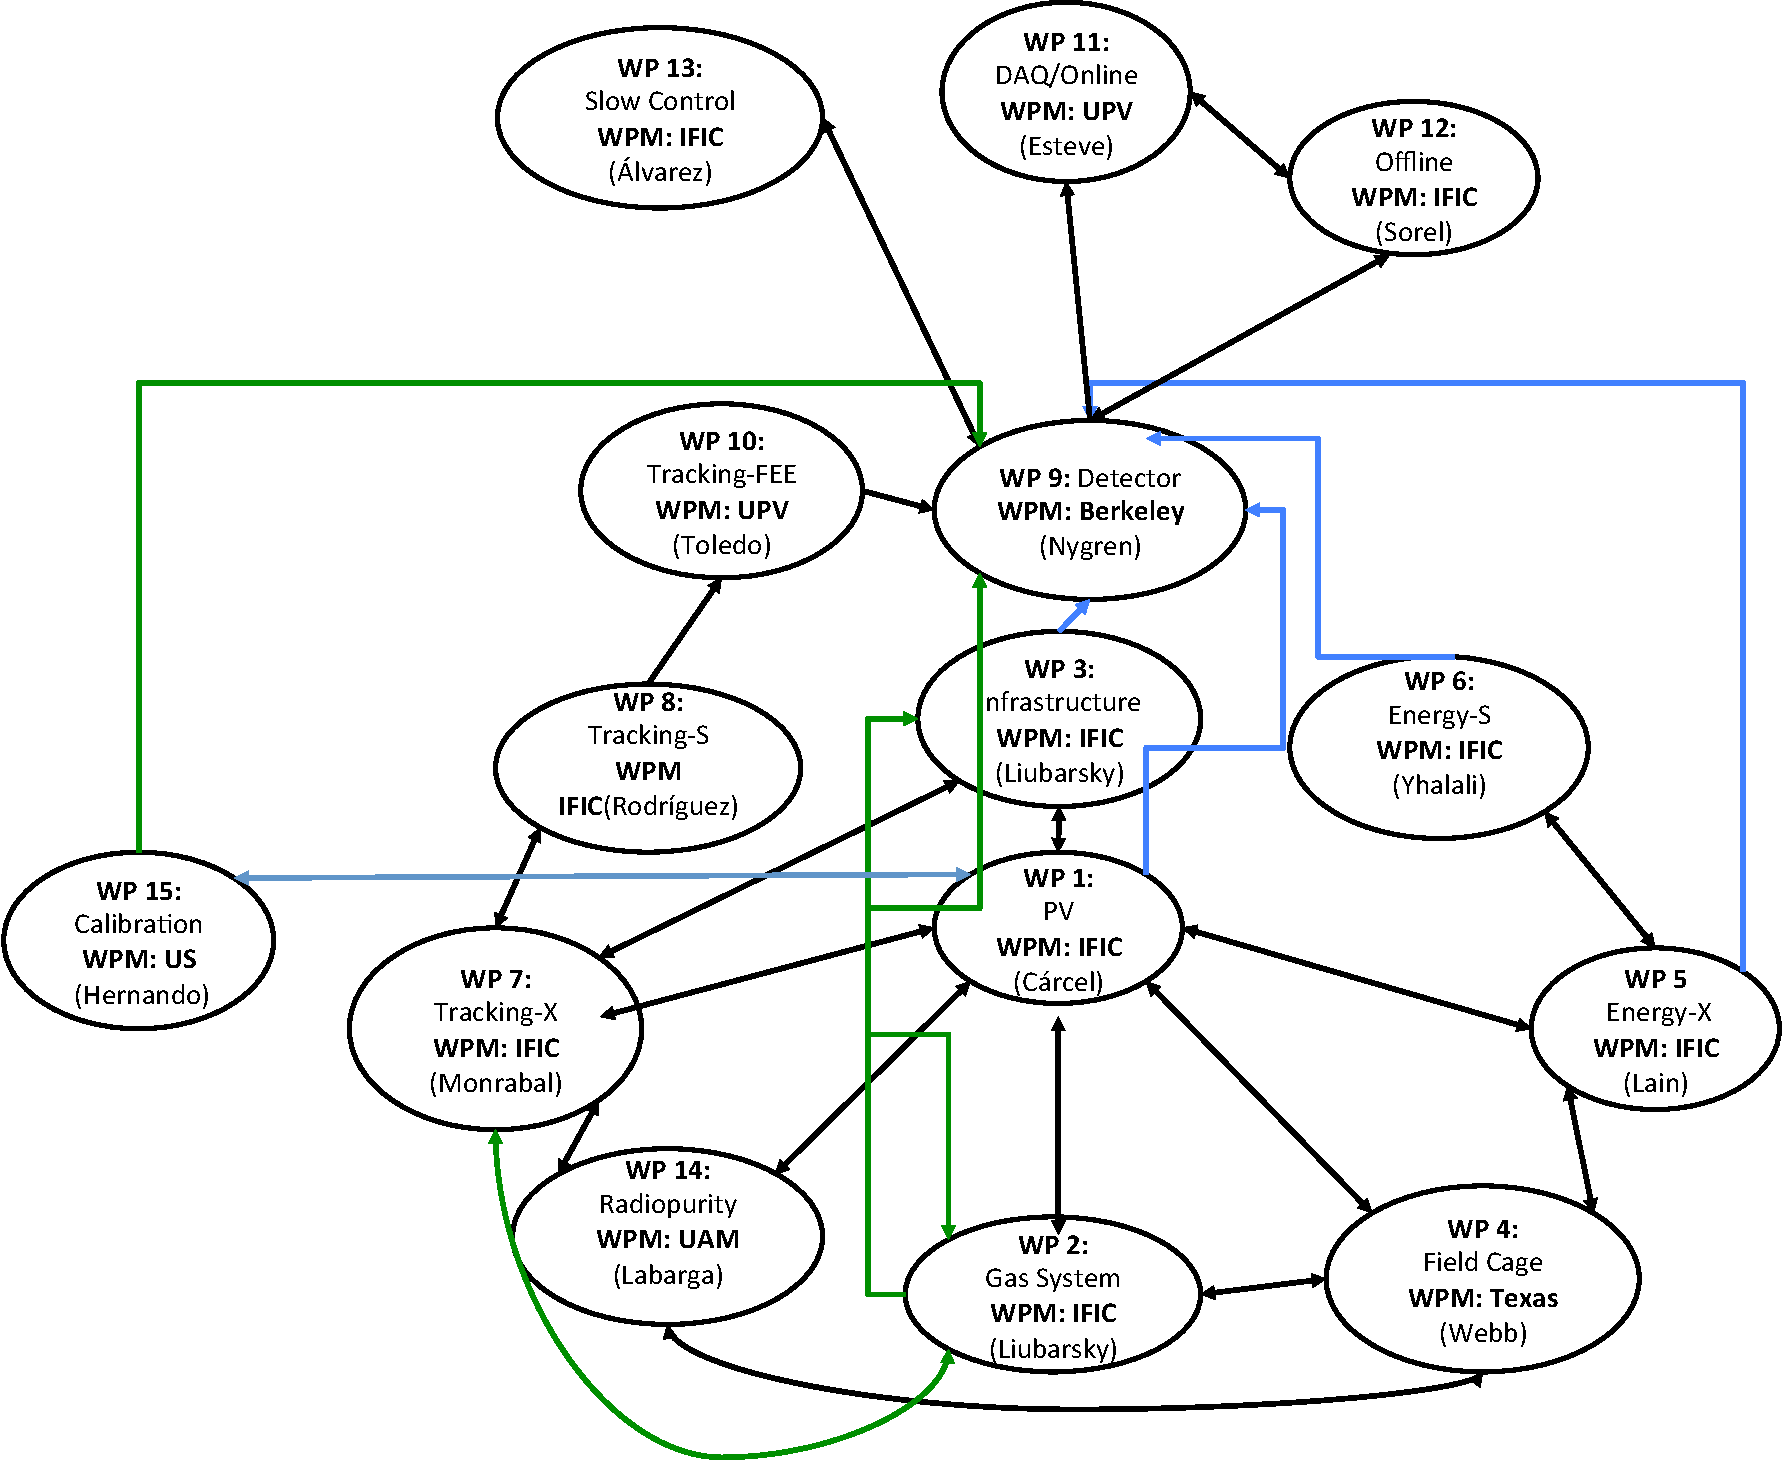
\includegraphics[width=0.75\textwidth]{img/PMP.pdf}
\end{center}
\caption{\label{Fig:PMP}Structure of work packages}
\end{figure}
%
%%\begin{figure}[h!]
%%\begin{center}
%%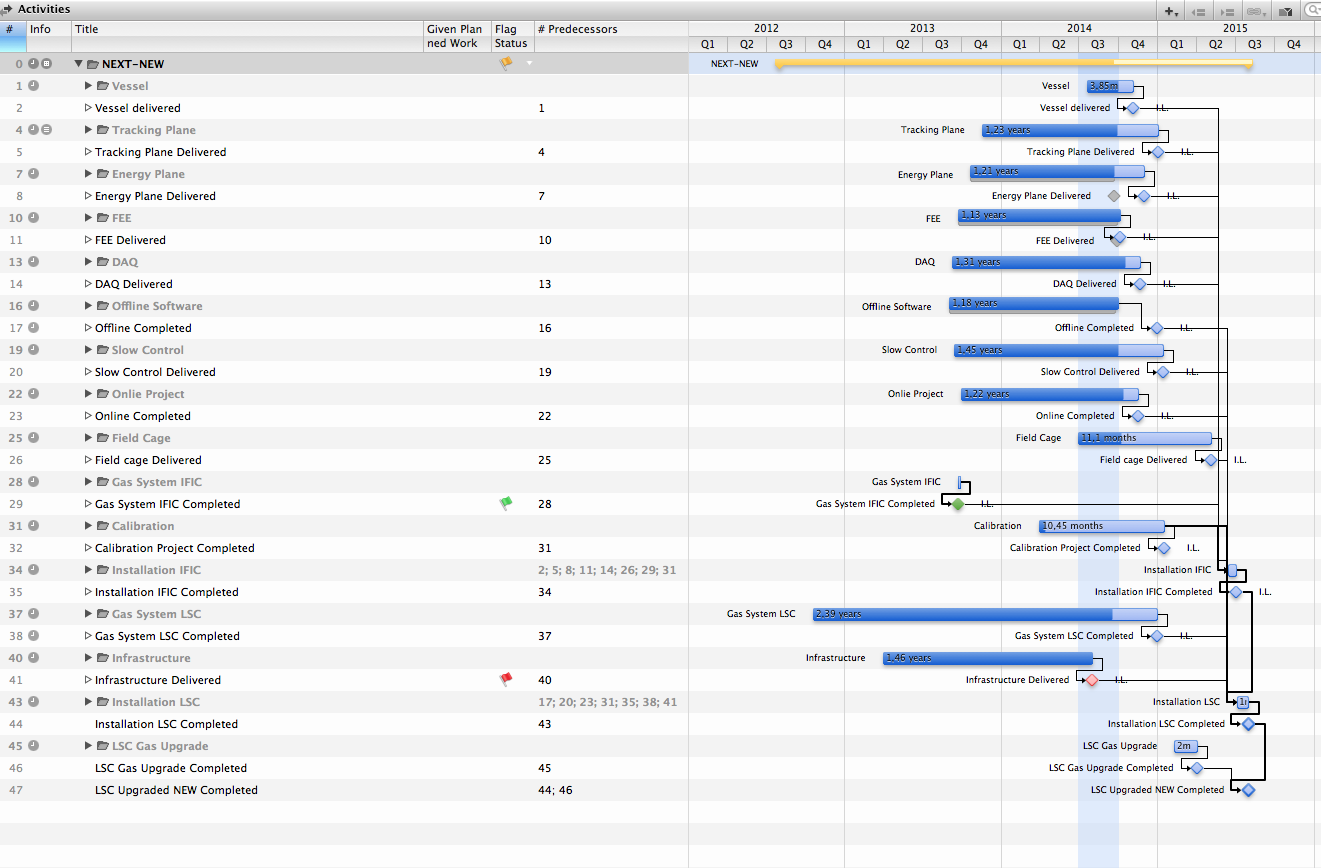
\includegraphics[width=0.99\textwidth]{img/Merlin_NEW.png}
%%\end{center}
%%\caption{\label{Fig:Gantt} Gantt chart for the NEW project (up to installation at the LSC)}
%%\end{figure}
%%
%\begin{figure}[h!]
%\begin{center}
%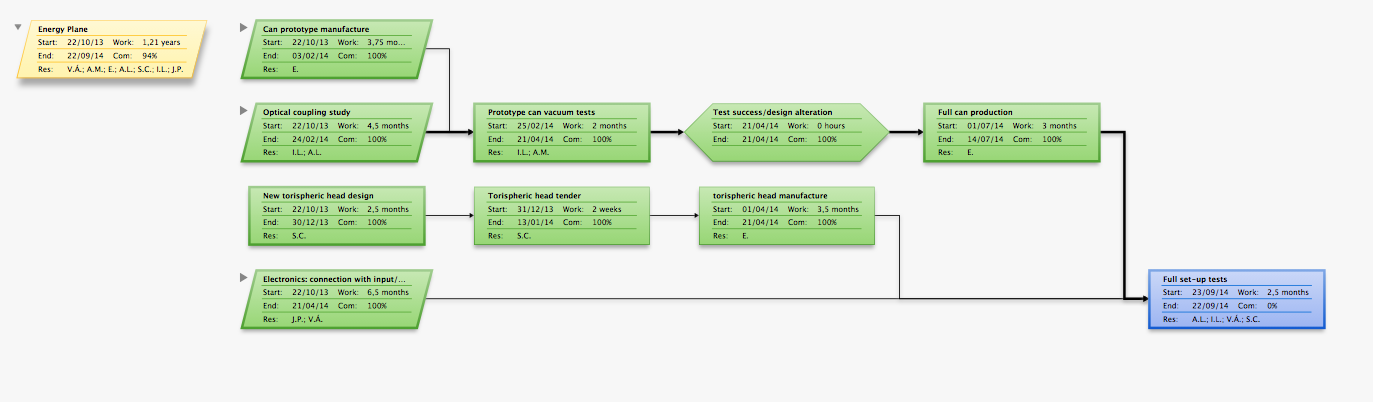
\includegraphics[width=0.99\textwidth]{img/EPG.png}
%\end{center}
%\caption{\label{Fig:NFC} Project description for the NEW Energy Plane (up to installation at the LSC)}
%\end{figure}

The different objectives described in the previous sections (as well as those of the ENG and CALREC sub projects) are integrated in the NEXT Project Management Plan (PMP, see Figure \ref{Fig:PMP}). 
The PMP coordinates the construction of the NEW and NEXT-100 detectors. It is under the direct supervision of the Spokesperson (SP) and the Project Manager (PM). The PM of NEXT is Dr. I. Liubarsky, part of the IFIC group.

The PMP defines a set of Working Packages (WP) and follows the progress of each one, monitors deliverables and dead lines and keeps track of invested resources including personnel. It also identifies potential show-stoppers and synergies (and possible conflicts) between the different projects and optimises the sharing of resources. 
%Figure \ref{fig.Gantt} shows an example of the Gantt chart for the whole NEW project, up to installation at the LSC. 
%The objectives defined for the different sub projects match the various WP in the PMP, as can be seen in Figure \ref{Fig:PMP}. 

The methodology of each WP includes: a) the definition of the associated tasks; b) the identification of the resources needed; c) the temporal organisation of the tasks; d) the definition of milestones and the deliverables associated to them. Each WP has a leader, which reports directly to the PM. The progress of each WP is reviewed on a weekly basis. Milestones and potential showstoppers are discussed, and the tracking charts updated if needed. The PMP is reviewed every six months by the LSC scientific committee.  

%Figure \ref{Fig:NFC} summarises the project description for the NEW Energy Plane as an example of the protocol followed for each system (field cage, tracking plane, etc). We also illustrate the methodology use for the chain production of various subsystems, describing the
%production of the PMT cans. The first step was the construction of a set of prototypes, which allowed us to improve the initial design (for example using brazing rather than the initial idea of CF gaskets) and certify correct operation. Test were conducted to ensure good light transmittance (this implied a lengthy search to find the optimal optical glue to couple the PMT quartz window to the PMT can sapphire window), vacuum tightness and no sparks at the bases. Finally, each one of the parts (copper stock, brazing stock, bolts, windows) were screened to ensure radio purity. The companies in charge of manufacturing the PMT cans, procuring the sapphire window, and coating the window with ITO were identified, costs secured, and delivery times specified. The protocol to coat the windows with TPB (at the italian laboratory of LNGS) was also specified. With all the above elements, the PMT can chain is defined, and then exercised with the production of 12 PMT cans for NEW. We expect to identify and correct any problem, and optimise the procedure during the process, which has already started. Once certified, the production of 60 PMT cans for NEXT-100 can proceed in a robust and predictable way. 
%
%Analogously the tracking plane subsystems include: The sensors themselves (SiPMs), which we have extensively tested. The flexible kapton boards (KDBs), whose design has already been certified, after a successful pre-production. The in-chamber cables which connect from the KDB to the feedthrough. The out-camber cables, which connect to the electronics. The feedthrough itself, which has already been successfully tested, showing a negligible leak rate. Almost every component of the NEXT tracking plane is a new technological development, including the KDBs which allow large matrices of SIPMs to be used as optical pixels and the feedthrough, which uses an innovative, yet affordable (and radio clean) technology. On the other hand, we have experienced few problems, and the system scales up nicely to the larger NEXT-100 detector (in short: we just need to mass-produced more KDBs and more feedthroughs). 

%From the methodological point of view, the commissioning and operation of NEW is also an essential ingredient for the success of NEXT-100. The operation of NEW will allow us to: a) fully test the dynamics of detector and its stability (as we have done with DEMO, after more than two years of continuous operation); test the entire signal chain, from sensor to digitisation; c) calibrate the detector and assess its performance. Such {\em system} evaluation will allow to identify and correct any design or implementation problem before starting the construction of NEXT-100. 

